\chapter{More Advanced Error Analysis}

\section{Objectives}

\begin{enumerate}
    \item To understand the concept of the random error.
    \item To study the propagation of errors from measured to derived quantities.
\end{enumerate}

\section{Introduction}

In the first chapter on errors, in the section on errors on time measurement, we found that the error on time measurement in our lab is almost certainly dominated by the reaction time of the observer. And, to determine this error, one method we suggested was to determine the time period many times and find the spread in the readings, using a measure called the standard deviation. The standard deviation is used in statistics to measure the characteristic spread of a random variable. The question then arises: What is a random variable? We will investigate this question in this chapter. 

The other matter we will address ourselves to in this chapter is that of propagation of errors. You will have noticed that in the earlier chapter on errors, we spoke at length on the errors on the observations themselves, e.g. the length $l$, or obtained by a simple operation from the observations, e.g. the time period $T$, but we said nothing about how this may affect quantity derived from these observations, e.g. the acceleration due to gravity $g$. It is clear that how certain we are of the time period and the length will affect how certain we are of $g$. In other words the errors on $l$ and $T$ will \textit{propagate} to $g$. How error propagates from observed quantities to derived quantities is the second subject of this chapter. 

\section{Random Errors}

To understand this, let us imagine trying to make a large number of tiles, by a manually operated machine. It is clear that though the tiles will be similar to each other, no two will be identical. The differences will be of various kinds, appearance, mass, edge length, etc. Since we want to look at the tiles through the eye of a physicist, let us concentrate on measurable quantities; we could choose edge length or mass; let us choose mass. 

The mass of a tile is what we call a \textit{random variable}, because the mass of one tile is different from that of another in a random manner (in spite of the template which tends of make them similar). If we want to find the characteristic mass of the tiles, we can weigh a number of them and find the average. However, what we are after is how different the tiles are from each other; so the mean won't do. What we could do, to begin with, is weigh a large number of them, and note them down. If we look carefully at the numbers, we will see that there is a spread. We see that numbers close to each other don't indicate much of a difference, and we'd like to think of them together. A powerful way to represent neighbouring readings together while highlighting the difference between distant readings is to draw a histogram. 
\subsection{Histogram}

In a histogram, we put the readings in a number of bins, i.e. we put all the readings in a certain range in the same bin, and we have a number of such bins to cover all the readings. There is no formula for the number of bins, but what we want a large-enough number of bins to see how the population differs from that in the others as we move across the readings, i.e. we want to see the pattern in the variation of the readings. 

The figure below shows a typical histogram, for --- readings of the mass of ---.

The bell-like shape of the pattern is characteristic. It is described by a famous mathematical function called the Gaussian. What we find is that whenever the variation from one reading to another is caused by a large number of factors unconnected with each other, this shape arises naturally. This is true in our example of the masses of a collection of tiles made with the same template. It is also true of the masses of group of human beings belonging to the same population, e.g. urban Punjabis. 

It is clear from the way we have arrived at the histogram that its width is determined by the spread of the readings. The mean does not contain information on this width; in fact what we are looking for is precisely how far the readings are, on the average, from the mean. If we imagine two artisans making the tiles, one a master who is able to achieve greater consistency and the other an apprentice, it ought to be clear that the histogram of the masses of the master's tiles will be narrower than that of the apprentice's tiles.

One way to characterise the spread of the masses might be to find the difference in mass between the heaviest tile and lightest tile. But there is something unsatisfactory about this because we are allowing the outliers to characterise and entire. What we would like to do is use all the readings to characterise the spread. This is done by the \textit{standard deviation} $\sigma$, which is given by the formula

\begin{equation}
    \sigma = \sqrt{\frac{\sum_{i=1}^{n} (x_i - \overline{x})^2}{n}},
\end{equation}

where $x_i$ is a reading, $\overline{x}$ is the mean, and $n$ is the number of readings.

For a Gaussian distribution of readings, i.e. a distribution the envelope of whose histogram is a Gaussian, about $68 \%$ of the readings are found between $x = \overline{x} - \sigma$ and $x = \overline{x} + \sigma$. Thus an arbitrary reading has a 68\% likelihood that an individual measurement will fall within one standard deviation $(\pm\sigma_x)$ of the mean\footnote{Keep in mind, however, the example of superluminal neutrinos we gave earlier: in that case, the error was \textit{assumed} to be random, and their precise data led them to a false positive. The true error turned out to be systematic, leading to \textit{different (and larger) error bars}!}. 


\begin{question}
    \paragraph{Question:} In the last paragraph we have gone from the fraction of readings in a certain range to a probability of an arbitrary reading's having a certain value. Go through this carefully and understand the argument.

    \paragraph{Question:} Do some research to find out what fraction of the readings are found in the range $\pm 2\sigma$ and $\pm 3 \sigma$ from the mean. 
\end{question}

When the significant source of error is considered to be random and the distribution is a Gaussian, random error associated with the reading is some factor times $\sigma$, the factor depending on how much confidence we wish to associate with our reading. If we choose $\sigma$ as our error -- this is a common choice -- the confidence associated with the reading is $68 \%$. 

\textbf{A note on statistics:} Consider two sets of measurements of the acceleration due to gravity:

\begin{table}[!htb]
\parbox{.45\linewidth}{
\centering
\begin{tabular}{cc}
\hline
\textbf{S. No.}&$\bm{g}\,\, (ms^{-2})$\\
\hline
1&$9.80\pm0.01$\\
2&$0.70\pm0.01$\\
3&$18.90\pm0.01$\\
4&$15.60\pm0.01$\\
5&$4.10\pm0.01$\\
\hline
Mean&$9.82\pm0.01$\\
\hline
\end{tabular}
\caption{Measurement of $g$ (Set 1)}
}
\hfill
\parbox{.45\linewidth}{
\centering
\begin{tabular}{cc}
\hline
\textbf{S. No.}&$\bm{g}\,\, (ms^{-2})$\\
\hline
1&$9.83\pm0.01$\\
2&$9.80\pm0.01$\\
3&$9.82\pm0.01$\\
4&$9.84\pm0.01$\\
5&$9.83\pm0.01$\\
\hline
Mean&$9.82\pm0.01$\\
\hline
\end{tabular}
\caption{Measurement of $g$ (Set 2)}
}
\end{table}

It would obviously be wrong to go simply by the mean and say that both these sets of data were equally reliable. In fact, stating the mean of the first set as the acceleration due to gravity \textbf{doesn't make sense}. 

Suppose we compared the mean of a data set to its \textit{dispersion} about the mean. If this is small, we could then say that there is some ``true'' value and that all the different values we measured occurred due to random fluctuations about this ``true'' value. Since the fluctuations are random, we could assume that they average out to zero, leaving us with a closer estimate to the ``true'' value than any individual reading.

\begin{question}
\paragraph{Question:} In above sets of data (with standard deviations of $7.6\,\,ms^{-2}$ and $0.02\,\,ms^{-2}$ respectively), does the quoted error of $\pm 0.01\,\, ms^{-2}$ make sense
\begin{enumerate}
    \item For Set 1?
    \item For Set 2?
    \item For Both?
    \item For Neither?
\end{enumerate}
Justify your answer quantitatively.
\end{question}

\begin{imp}
The two errors in the lab you will encounter that you cannot remove are \textbf{least count errors} and \textbf{random errors}. Remember to always compare them and \textbf{\textit{take the larger value}}. In Set 1 it makes no sense to say $g$ is specified to $(9.82\pm0.01)\,ms^{-2}$, since all of the values are much farther away than that!
\end{imp}

\begin{question}
\begin{enumerate}
    \item \textbf{Question:} Multiple measurements with the same instrument increases the
    \begin{enumerate}
        \item Accuracy
        \item Precision
        \item Both
    \end{enumerate}
    
    \item \textbf{Question:} Consider the following data-table~\\
    \begin{tabular}{cccccc}
    \hline
    \textbf{S. No.}&1&2&3&4&5\\
    \hline
    \textbf{Time Period} ($s$)& $1.2\pm0.1$&$1.2\pm0.1$&$1.2\pm0.1$&$1.2\pm0.1$&$1.2\pm0.1$\\
    \hline
    \end{tabular}~\\~\\
    The standard deviation is $0.0$. Would it be right to say that $T_\text{avg} = 1.2\pm 0.0$?
\end{enumerate}
\end{question}

However, keep in mind there are many cases where the mean  \textbf{does not} represent some true value\footnote{For example, even if the average number of siblings every student has is $1.574$, there is no student who has a non-integer number of siblings.}. There are also cases where the standard deviation contains physical information. Such cases are usually a result of statistical phenomena.

\begin{tip}
\begin{enumerate}
    \item In a coin-toss experiment with a large number of tosses, $\sigma$ gives you a measure of the bias of the coin.
    \item In a random walk, $\sigma$ can be a measure of the diffusion coefficient $D$.
    \item In shot-noise --  the statistical fluctuations of current due to the actual number of electrons flowing in the conductor per unit time -- $\sigma$ gives you a measure of Boltzmann's constant $k_B$.
\end{enumerate}
\end{tip}






\subsection{Reporting Errors}
\subsubsection{Significant figures}

The significant figures of a number are the digits in its representation that contribute to the precision of the number. In practice, we assume that all digits used to write a number are significant (except leading zeroes\footnote{Non-leading zeros are considered to be significant. If you write a number as 1,200, we assume there are four significant digits. If you only mean to have two or three, then it is best to use scientific notation: $1.2 \times 10^3$ or $1.20 \times 10^3$ . Leading zeros are not considered significant: 0.55 and 0.023 have just two significant figures.}).

\textbf{Results of simple calculations should not increase the number of significant digits}. Calculations transform our knowledge; they do not increase it! The rounding should be performed at the final step of a calculation to prevent rounding errors at intermediate steps from propagating through your work but \textbf{only} one or two
extra digits suffice to prevent this.

If you measure a value on a two-digit digital meter to be 1.0 and another value to be 3.0, it is incorrect to say that the ratio of these measurements is 0.3333333. The two values are not exact numbers with infinite precision. Since they each have two significant digits, the correct number to write down is 0.33\footnote{If this is an intermediate result, then 0.333 or 0.3333 are preferred, but the final result must have two significant digits.}.

\begin{imp}
\textbf{Do not write significant figures beyond the first digit of the error on the quantity}. Giving more precision than this to a value is not only irrelevant, \textit{it is misleading}.\\

If you're told you're using FAR too many digits, please do not try to use the excuse, ``That's what the computer gave me.'' \textbf{You} are in charge of presenting your results, not the computer!
\end{imp}


\subsubsection{Error propagation}

Experiments worth carrying out rarely measure only one quantity. Typically we measure two or more quantities and then `fold' them together in some equation or equations to determine some other quantity that we believe to depend on them. It is thus imperative that we understand how uncertainties in certain measured quantities `propagate' into other derived quantities.

For our analysis, let us assume that

\begin{itemize}
    \item $x$ and $y$ are measured quantities with uncertainties $\delta x$ and $\delta y$ respectively. These errors are considered to be \textbf{uncorrelated}, meaning that $\delta x$ and $\delta y$ are independent\footnote{For example, the precision of measuring the length of your simple pendulum has no effect on the precision of measuring time.}.
    
    \item $c$ is a constant known to known absolutely precisely (or with negligible uncertainty).
    
    \item $z$ is a quantity \textit{derived} from $x$ and $y$ and possessing a `propagated' uncertainty $\delta z$.
\end{itemize}

The formulae used to compute errors are usually not completely understood: a variety of different formulae are used in different cases, and the reasons \textbf{why} are usually lost on students. It turns out that there is only \textbf{one} way to add (uncorrelated) errors, which one can manipulate to get the rest:

\begin{imp}
If $z = x + y$, their (uncorrelated) errors add \textbf{in quadrature}:
\begin{equation}
    \delta z = \sqrt{\left(\delta x\right)^2+\left(\delta y\right)^2}
    \label{quadrature}
\end{equation}
\end{imp}

The reason for errors adding in quadrature is one that comes from statistics; it is essential that the errors be \textbf{independent} of each other (uncorrelated)\footnote{It also makes sense:  errors could be positive and some negative, simply adding them could conceivably give a smaller number (or even zero!). Thus, the next best thing is to add their \textit{squares}. }

Here is another motivation\footnote{This is \textbf{not} an explanation of why this is true!}: you could imagine two uncorrelated measurements to represent two axes ($x$ and $y$) that are orthogonal to each other (see Figure (\ref{fig:quadrature}). Imagine that you want to specify a point $z = (x,y)$: given that there is an uncertainty in both the coordinates $x$ and $y$, the point $z$ is uncertain \textbf{at most} by $\delta z = \sqrt{\left(\delta x\right)^2+\left(\delta y\right)^2}$.

\begin{figure}
    \centering
    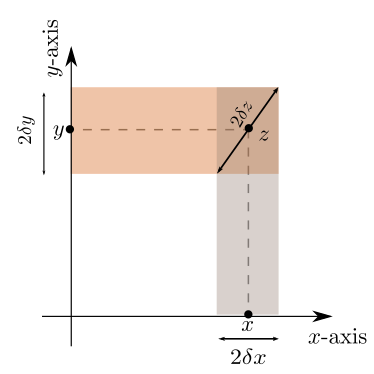
\includegraphics[scale=0.5]{figs/quadrature.png}
    \caption{Two points $(x,0)$ and $(0,y)$, with uncertainties $\delta x$ and $\delta y$ respectively, can be summed to get a point $z=(x,y)$ with uncertainty $\delta z$. }
    \label{fig:quadrature}
\end{figure}

This formula can then be used to get the uncertainties of more complicated relations. For example, consider $z = xy$. In this case, the two quantities are \textbf{multiplied}, and so we can't use the above formula as is. We could, however, take the log, and get $\log{z} = \log{x} + \log{y}$. This is of the form $u = v + w$. We could then apply Equation (\ref{quadrature}), and find that $$\delta \left(\log{z}\right) = \sqrt{\left(\delta \left(\log{x}\right)\right)^2 + \left(\delta \left(\log{y}\right)\right)^2}$$

The uncertainty in $\log{z}$ can easily be related by taking the derivative\footnote{A differential is by definition the variation of function when its parameter changes by a small amount. We want to find how much $\log{z}$ changes when $z$ changes by $\delta z$. We use $\delta$ instead of $\dd$, since the variation is not truly \textit{infinitesimal}.}.

\begin{equation*}
    \dd({\log{z}}) = \frac{\dd z}{z} \quad \implies \quad \delta (\log{z}) = \frac{\delta z}{z}
\end{equation*}

Thus, 

\begin{equation}
    \frac{\delta z}{z} = \sqrt{\left(\frac{\delta x}{x}\right)^2 + \left(\frac{\delta y}{y}\right)^2}
\end{equation}

\begin{tip}
The following rules should exhaust most of the common cases that you will be exposed to in your undergraduate labs. Everything here can be generalised simply to a a \textit{set} of measurements $x_i$ with uncertainties $\delta x_i$.

\begin{enumerate}
    \item \textbf{Addition or subtraction by a constant:} If $z = c \pm x$, then 
    \begin{equation}
        \delta z = \delta x
    \end{equation}
    
    
    \item \textbf{Multiplication by a constant:} If $z = c x$, then 
    \begin{equation}
        \delta z = c\delta x
    \end{equation}
    
    \item \textbf{Addition or subtraction of two measured quantities:} If $z = x \pm y$, then 
    
    \begin{equation}
        \delta z = \sqrt{(\delta x)^2 +(\delta y)^2}
    \end{equation}
    
    \item \textbf{Multiplication or division of two measured quantities:} If $z = xy$ or $z = \frac{x}{y}$, then 
    
    \begin{equation}
        \frac{\delta z}{z} = \sqrt{\left(\frac{\delta x}{x}\right)^2 + \left(\frac{\delta y}{y} \right)^2}
        \label{relerror}
    \end{equation}
    
    \item \textbf{A measured quantity raised to a power:} If $z = x^c$, then
    
    \begin{equation}
        \frac{\delta z}{z} = c \frac{\delta x}{x}
        \label{powerror}
    \end{equation}
    
\end{enumerate}
\end{tip}

\begin{question}
\paragraph{Question:} Prove Equation (\ref{powerror}).~\\

\paragraph{Question:} If $z = x^2 = x \times x$, we get different answers if we use the Power Rule (Equation (\ref{powerror})) or the Product Rule (Equation (\ref{relerror})). Which of the two is correct? Why? ~\\

\paragraph{Question:} Calculate the uncertainty in $z$ if
\begin{enumerate}
    \item $z = \frac{1}{x}$
    \item $z = \frac{x}{1+x}$
    \item $z = \frac{x}{x+y}$
\end{enumerate}
\paragraph{Hint:} The last one is slightly hard. You will first write it as $z = \frac{1}{1 + u}$, where $u = y/x$. Then, calculate $\delta z$ in terms of $\delta u$, and only then $\delta u$ in terms of $\delta x$ and $\delta y$.
\end{question}
